\documentclass[11pt,a4paper,]{article}
\usepackage{lmodern}

\usepackage{amssymb,amsmath}
\usepackage{ifxetex,ifluatex}
\usepackage{fixltx2e} % provides \textsubscript
\ifnum 0\ifxetex 1\fi\ifluatex 1\fi=0 % if pdftex
  \usepackage[T1]{fontenc}
  \usepackage[utf8]{inputenc}
\else % if luatex or xelatex
  \usepackage{unicode-math}
  \defaultfontfeatures{Ligatures=TeX,Scale=MatchLowercase}
\fi
% use upquote if available, for straight quotes in verbatim environments
\IfFileExists{upquote.sty}{\usepackage{upquote}}{}
% use microtype if available
\IfFileExists{microtype.sty}{%
\usepackage[]{microtype}
\UseMicrotypeSet[protrusion]{basicmath} % disable protrusion for tt fonts
}{}
\PassOptionsToPackage{hyphens}{url} % url is loaded by hyperref
\usepackage[unicode=true]{hyperref}
\hypersetup{
            pdftitle={Analysing players of LaLiga Football Tournament to find the best player in each Position},
            pdfborder={0 0 0},
            breaklinks=true}
\urlstyle{same}  % don't use monospace font for urls
\usepackage{geometry}
\geometry{a4paper, centering, text={16cm,24cm}}
\usepackage[style=authoryear-comp,]{biblatex}
\addbibresource{references.bib}
\usepackage{longtable,booktabs}
% Fix footnotes in tables (requires footnote package)
\IfFileExists{footnote.sty}{\usepackage{footnote}\makesavenoteenv{long table}}{}
\IfFileExists{parskip.sty}{%
\usepackage{parskip}
}{% else
\setlength{\parindent}{0pt}
\setlength{\parskip}{6pt plus 2pt minus 1pt}
}
\setlength{\emergencystretch}{3em}  % prevent overfull lines
\providecommand{\tightlist}{%
  \setlength{\itemsep}{0pt}\setlength{\parskip}{0pt}}
\setcounter{secnumdepth}{5}

% set default figure placement to htbp
\makeatletter
\def\fps@figure{htbp}
\makeatother


\title{Analysing players of LaLiga Football Tournament to find the best player in each Position}

%% MONASH STUFF

%% CAPTIONS
\RequirePackage{caption}
\DeclareCaptionStyle{italic}[justification=centering]
 {labelfont={bf},textfont={it},labelsep=colon}
\captionsetup[figure]{style=italic,format=hang,singlelinecheck=true}
\captionsetup[table]{style=italic,format=hang,singlelinecheck=true}


%% FONT
\RequirePackage{bera}
\RequirePackage[charter,expert,sfscaled]{mathdesign}
\RequirePackage{fontawesome}

%% HEADERS AND FOOTERS
\RequirePackage{fancyhdr}
\pagestyle{fancy}
\rfoot{\Large\sffamily\raisebox{-0.1cm}{\textbf{\thepage}}}
\makeatletter
\lhead{\textsf{\expandafter{\@title}}}
\makeatother
\rhead{}
\cfoot{}
\setlength{\headheight}{15pt}
\renewcommand{\headrulewidth}{0.4pt}
\renewcommand{\footrulewidth}{0.4pt}
\fancypagestyle{plain}{%
\fancyhf{} % clear all header and footer fields
\fancyfoot[C]{\sffamily\thepage} % except the center
\renewcommand{\headrulewidth}{0pt}
\renewcommand{\footrulewidth}{0pt}}

%% MATHS
\RequirePackage{bm,amsmath}
\allowdisplaybreaks

%% GRAPHICS
\RequirePackage{graphicx}
\setcounter{topnumber}{2}
\setcounter{bottomnumber}{2}
\setcounter{totalnumber}{4}
\renewcommand{\topfraction}{0.85}
\renewcommand{\bottomfraction}{0.85}
\renewcommand{\textfraction}{0.15}
\renewcommand{\floatpagefraction}{0.8}


%\RequirePackage[section]{placeins}

%% SECTION TITLES


%% SECTION TITLES (NEW: Changing sections and subsections color)
\RequirePackage[compact,sf,bf]{titlesec}
\titleformat*{\section}{\Large\sf\bfseries\color[rgb]{0.13, 0.67, 0.8 }}
\titleformat*{\subsection}{\large\sf\bfseries\color[rgb]{0.13, 0.67, 0.8 }}
\titleformat*{\subsubsection}{\sf\bfseries\color[rgb]{0.13, 0.67, 0.8 }}
\titlespacing{\section}{0pt}{2ex}{.5ex}
\titlespacing{\subsection}{0pt}{1.5ex}{0ex}
\titlespacing{\subsubsection}{0pt}{.5ex}{0ex}


%% TITLE PAGE
\def\Date{\number\day}
\def\Month{\ifcase\month\or
 January\or February\or March\or April\or May\or June\or
 July\or August\or September\or October\or November\or December\fi}
\def\Year{\number\year}

%% LINE AND PAGE BREAKING
\sloppy
\clubpenalty = 10000
\widowpenalty = 10000
\brokenpenalty = 10000
\RequirePackage{microtype}

%% PARAGRAPH BREAKS
\setlength{\parskip}{1.4ex}
\setlength{\parindent}{0em}

%% HYPERLINKS
\RequirePackage{xcolor} % Needed for links
\definecolor{darkblue}{rgb}{0,0,.6}
\RequirePackage{url}

\makeatletter
\@ifpackageloaded{hyperref}{}{\RequirePackage{hyperref}}
\makeatother
\hypersetup{
     citecolor=0 0 0,
     breaklinks=true,
     bookmarksopen=true,
     bookmarksnumbered=true,
     linkcolor=darkblue,
     urlcolor=blue,
     citecolor=darkblue,
     colorlinks=true}

\usepackage[showonlyrefs]{mathtools}
\usepackage[no-weekday]{eukdate}

%% BIBLIOGRAPHY

\makeatletter
\@ifpackageloaded{biblatex}{}{\usepackage[style=authoryear-comp, backend=biber, natbib=true]{biblatex}}
\makeatother
\ExecuteBibliographyOptions{bibencoding=utf8,minnames=1,maxnames=3, maxbibnames=99,dashed=false,terseinits=true,giveninits=true,uniquename=false,uniquelist=false,doi=false, isbn=false,url=true,sortcites=false}

\DeclareFieldFormat{url}{\texttt{\url{#1}}}
\DeclareFieldFormat[article]{pages}{#1}
\DeclareFieldFormat[inproceedings]{pages}{\lowercase{pp.}#1}
\DeclareFieldFormat[incollection]{pages}{\lowercase{pp.}#1}
\DeclareFieldFormat[article]{volume}{\mkbibbold{#1}}
\DeclareFieldFormat[article]{number}{\mkbibparens{#1}}
\DeclareFieldFormat[article]{title}{\MakeCapital{#1}}
\DeclareFieldFormat[article]{url}{}
%\DeclareFieldFormat[book]{url}{}
%\DeclareFieldFormat[inbook]{url}{}
%\DeclareFieldFormat[incollection]{url}{}
%\DeclareFieldFormat[inproceedings]{url}{}
\DeclareFieldFormat[inproceedings]{title}{#1}
\DeclareFieldFormat{shorthandwidth}{#1}
%\DeclareFieldFormat{extrayear}{}
% No dot before number of articles
\usepackage{xpatch}
\xpatchbibmacro{volume+number+eid}{\setunit*{\adddot}}{}{}{}
% Remove In: for an article.
\renewbibmacro{in:}{%
  \ifentrytype{article}{}{%
  \printtext{\bibstring{in}\intitlepunct}}}

\AtEveryBibitem{\clearfield{month}}
\AtEveryCitekey{\clearfield{month}}

\makeatletter
\DeclareDelimFormat[cbx@textcite]{nameyeardelim}{\addspace}
\makeatother

\author{\sf\Large\textbf{ Sneha Kharbanda}\\ {\sf\large Master of Business Analytics\\[0.5cm]} \sf\Large\textbf{ Dhruv Nirmal}\\ {\sf\large Master of Business Analytics\\[0.5cm]} \sf\Large\textbf{ Rohan Baghel}\\ {\sf\large Master of Business Analytics\\[0.5cm]} \sf\Large\textbf{ Xianghe Xu}\\ {\sf\large Master of Business Analytics\\[0.5cm]}}

\date{\sf\Date~\Month~\Year}
\makeatletter
\lfoot{\sf Kharbanda, Nirmal, Baghel, Xu: \@date}
\makeatother


%%%% PAGE STYLE FOR FRONT PAGE OF REPORTS

\makeatletter
\def\organization#1{\gdef\@organization{#1}}
\def\telephone#1{\gdef\@telephone{#1}}
\def\email#1{\gdef\@email{#1}}
\makeatother
  \organization{Monash University}

  \def\name{DBMS consultancy}

  \telephone{(03) 9905 2478}

  \email{questions@dbms.com}                 %NEW: New email addresss

\def\webaddress{\url{http://company.com/stats/consulting/}} %NEW: URl
\def\abn{12 377 614 630}                                    % NEW: ABN
\def\logo{
\includegraphics[width=6cm]{Figures/logo}}  %NEW: Changing logo
\def\extraspace{\vspace*{1.6cm}}
\makeatletter
\def\contactdetails{\faicon{phone} & \@telephone \\
                    \faicon{envelope} & \@email}
\makeatother

%%%% FRONT PAGE OF REPORTS

\def\reporttype{Report for}

\long\def\front#1#2#3{
\newpage
\begin{singlespacing}
\thispagestyle{empty}
\vspace*{-1.4cm}
\hspace*{-1.4cm}
\hbox to 16cm{
  \hbox to 6.5cm{\vbox to 14cm{\vbox to 25cm{
    \logo
    \vfill
    \parbox{6.3cm}{\raggedright
      \sf\color[rgb]{0.8, 0.7, 0.1 }    % NEW color 
      {\large\textbf{\name}}\par
      \vspace{.7cm}
      \tabcolsep=0.12cm\sf\small
      \begin{tabular}{@{}ll@{}}\contactdetails
      \end{tabular}
      \vspace*{0.3cm}\par
      ABN: \abn\par
    }
  }\vss}\hss}
  \hspace*{0.2cm}
  \hbox to 1cm{\vbox to 14cm{\rule{4pt}{26.8cm}\vss}\hss\hfill}  %NEW: Thicker line
  \hbox to 10cm{\vbox to 14cm{\vbox to 25cm{   
      \vspace*{3cm}\sf\raggedright
      \parbox{11cm}{\sf\raggedright\baselineskip=1.2cm
         \fontsize{24.88}{30}\color[rgb]{0, 0.29, 0.55}\sf\textbf{#1}}   % NEW: title color blue
      \par
      \vfill
      \large
      \vbox{\parskip=0.8cm #2}\par
      \vspace*{2cm}\par
      \reporttype\\[0.3cm]
      \hbox{#3}%\\[2cm]\
      \vspace*{1cm}
      {\large\sf\textbf{\Date~\Month~\Year}}
   }\vss}
  }}
\end{singlespacing}
\newpage
}

\makeatletter
\def\titlepage{\front{\expandafter{\@title}}{\@author}{\@organization}}
\makeatother

\usepackage{setspace}
\setstretch{1.5}

\usepackage{float}
\let\origfigure\figure
\let\endorigfigure\endfigure
\renewenvironment{figure}[1][2] {
    \expandafter\origfigure\expandafter[H]
} {
    \endorigfigure
}
\usepackage{booktabs}
\usepackage{longtable}
\usepackage{array}
\usepackage{multirow}
\usepackage{wrapfig}
\usepackage{float}
\usepackage{colortbl}
\usepackage{pdflscape}
\usepackage{tabu}
\usepackage{threeparttable}
\usepackage{threeparttablex}
\usepackage[normalem]{ulem}
\usepackage{makecell}
\usepackage{xcolor}


\begin{document}
\titlepage

\hypertarget{introduction}{%
\section{Introduction}\label{introduction}}

LaLiga, is the men's top professional football division of the Spanish football league system. It is contested by 20 teams, with the three lowest-placed teams at the end of each season being relegated to the Segunda División and replaced by the top two teams and a play-off winner in that division. According to UEFA's league coefficient rankings, La Liga has been the top league in Europe in each of the seven years from 2013 to 2019.

\hypertarget{research-question}{%
\subsection{Research Question}\label{research-question}}

In this report we are going to analyse the best player in each of the positions. The four positions are goalkeeper, forward, defender and midfielder. The data we have used provides information about each and every player in the league like goals scored, assists made, fouls committed etc. In each of the sections we will be using these variables to the best of our knowledge, to get the best player out of the 20 teams. For accurate comparison we have used a base research paper (\textcite{dellal2011comparison}).

\hypertarget{position-defender}{%
\section{Position: Defender}\label{position-defender}}

The motive of this section is to find out the \textbf{best defender} (defender : a defender is an outfield player whose primary roles are to stop attacks during the game and prevent the opposing team from scoring goals) in Laliga (Spanish football league), season 2019-2020 according to player stats. We will be analyzing different variables and going through different levels, to get the best defender out of the 20 teams.

We will try to find the best defender by going through different levels, the major one being, trying to find the player who has the most recoveries and clearances.

\begin{itemize}
\item
  Recovery - A recovery is recorded at the point where the player of the team beginning the possession touches the ball.
\item
  Clearance - When a player kicks the ball away from the goal they are defending.
\end{itemize}

We will only analyze players who have played more than \textbf{50\%} of the games, considering consistency is key factor for a 38 matches long league.

\begin{figure}[H]

{\centering 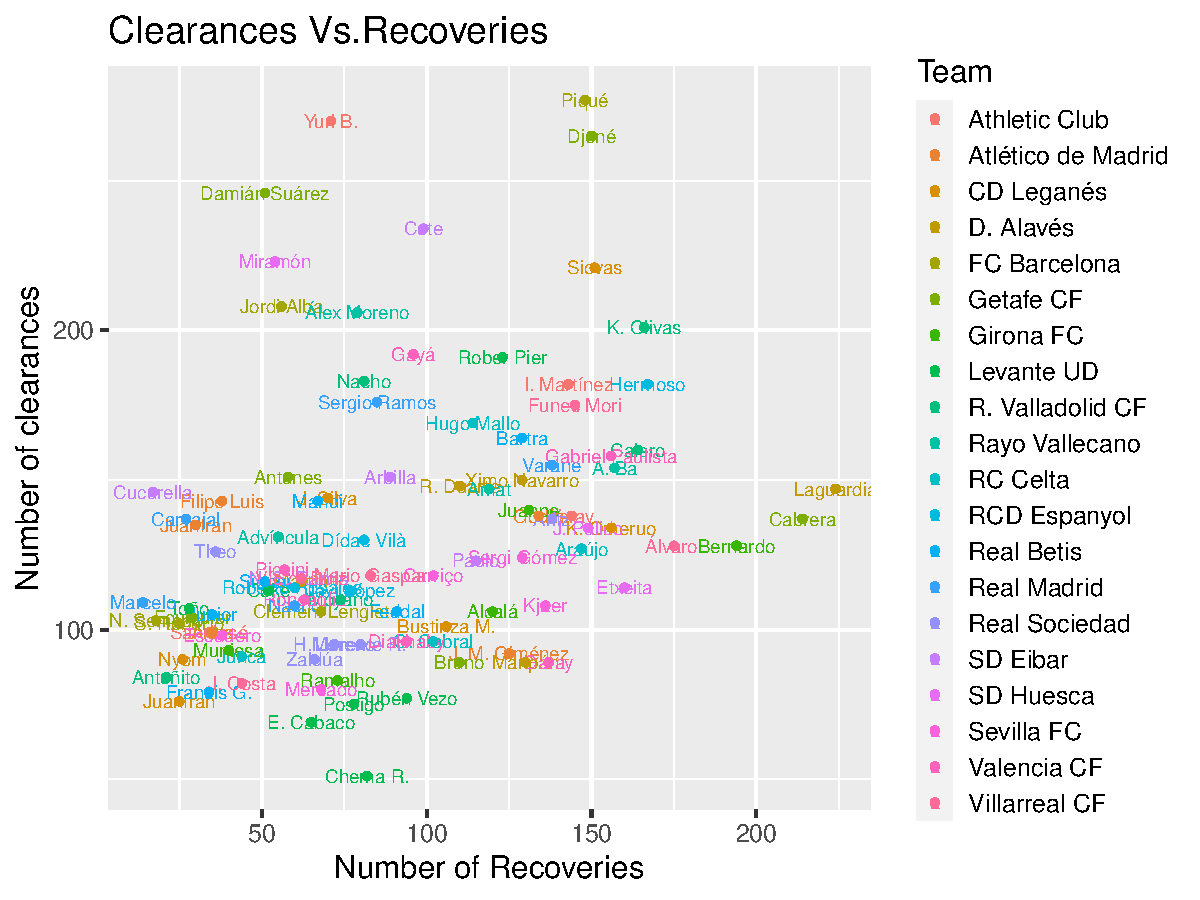
\includegraphics[width=0.8\linewidth]{Assignment-4-ETC5513_files/figure-latex/CvsR-1} 

}

\caption{Clearances vs Recoveries}\label{fig:CvsR}
\end{figure}

From \ref{fig:CvsR} we can say that \textbf{Pique} from \textbf{Barcelona} and \textbf{Laguardia} from \textbf{D. Alaves} have managed to do exceptionally well. Out of the two players, we will try to choose the best defender by bringing in more variables into the picture.

\begin{figure}[H]

{\centering 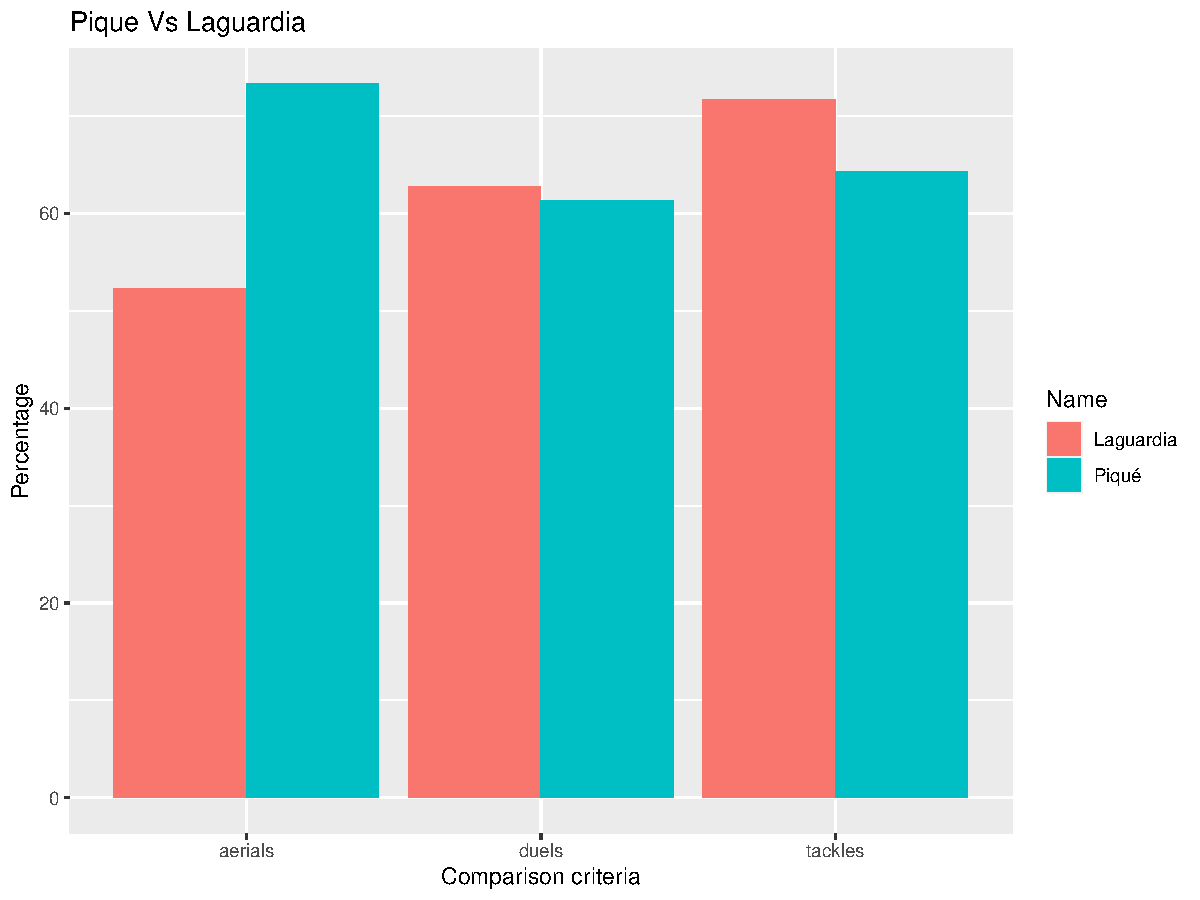
\includegraphics[width=0.8\linewidth]{Assignment-4-ETC5513_files/figure-latex/better1-1} 

}

\caption{Pique Vs Laguardia}\label{fig:better1}
\end{figure}

In the figure above \ref{fig:better1} we have calculated the percentage of successful tackles, duels and Aerial duels won by the each of the defender who came on top in \ref{fig:CvsR} i.e Pique and Laguardia. Laguardia top the charts between him and Pique in Successful tackles made and Duels won but the difference is bleak. Pique had \textbf{20\%} more Aerial duel success than Laguardia.

Seems like both of them are are still going to head to head. Now we have to judge them by number of mistakes made by them during the season.
\newpage

\begin{table}[H]

\caption{\label{tab:worse}Comparison of Pique and Laguardia (worse)}
\centering
\begin{tabular}[t]{l|l|r|r|r}
\hline
Name & Team & Goals.conceded.while.player.on.pitch & Yellow.Cards & Fouls.committed\\
\hline
Laguardia & D. Alavés & 44 & 12 & 26\\
\hline
Piqué & FC Barcelona & 30 & 6 & 24\\
\hline
\end{tabular}
\end{table}

From the table \ref{tab:worse} we can see Pique has made lesser mistakes in a match the while being on the field as compared to Laguardia. His team conceded lesser goals, he made lesser fouls which resulted him getting penalized less often. We can conclude from our analysis that Pique from Barcelona had the most impact as a defender. On top of that he was also able to contribute in the attack as he scored 4 goals for FC Barcelona.\\

\begin{table}[H]

\caption{\label{tab:unnamed-chunk-3}Goals scored by Pique}
\centering
\begin{tabular}[t]{l|l|r}
\hline
Name & Team & Goals.scored\\
\hline
Piqué & FC Barcelona & 4\\
\hline
\end{tabular}
\end{table}
\newpage

\hypertarget{position-forward}{%
\section{Position: Forward}\label{position-forward}}

\begin{itemize}
\item
  The aim of this section is to analyse which player is the best in the \emph{Forward position} (attacking player who is most responsible for scoring goals) in the LaLiga Tournament based on data from 2019-2020. The research paper \textcite{majewski2016identification} helped in guiding this analysis to the right path.
\item
  The analysis is done using goals scored, penalties scored, assists, success score, and yellow cards received by a player.
\end{itemize}

Goals Scored, Penalties Scored and Assists account for the most successful outcome given by a player in the Forward position.

\begin{table}[H]

\caption{\label{tab:Goals-Analysis}Top 5 forward position players for goals per game}
\centering
\begin{tabular}[t]{l|l|r|r}
\hline
Team & Name & goals\_per\_game & Goal\_rank\\
\hline
FC Barcelona & Messi & 1.5588235 & 1\\
\hline
RC Celta & Iago Aspas & 1.1481481 & 2\\
\hline
FC Barcelona & Suárez & 0.9393939 & 3\\
\hline
Real Madrid & Benzema & 0.8333333 & 4\\
\hline
Sevilla FC & Ben Yedder & 0.8285714 & 5\\
\hline
\end{tabular}
\end{table}

The table \ref{tab:Goals-Analysis} displays the Name and Team of the top 5 players in the forward position with the highest goals, penalties and assists per game. Messi from Team FC Barcelona holds the first rank in this analysis with an average of 1.55 goals per match, followed by lago Aspas and Suárez.

\begin{table}[H]

\caption{\label{tab:Success-Scores}Top 5 forward position players for Success Score}
\centering
\begin{tabular}[t]{l|l|r|r}
\hline
Team & Name & success\_score & Score\_rank\\
\hline
D. Alavés & Calleri & 10.029412 & 1\\
\hline
SD Huesca & Enric Gallego & 9.210526 & 2\\
\hline
CD Leganés & Carrillo & 8.937500 & 3\\
\hline
Atlético de Madrid & Morata & 8.666667 & 4\\
\hline
Rayo Vallecano & M. L. S. Trejo & 7.807692 & 5\\
\hline
\end{tabular}
\end{table}

As seen from the table \ref{tab:Success-Scores}, Calleri from team D. Alavés tops the table with a total success score of 10.02 followed by Enric Gallego and Carrillo The Success score in this table is calculated by adding the successful duels, tackles and aerial challenges by each player divided by the number of games they have played.

\begin{figure}[H]

{\centering 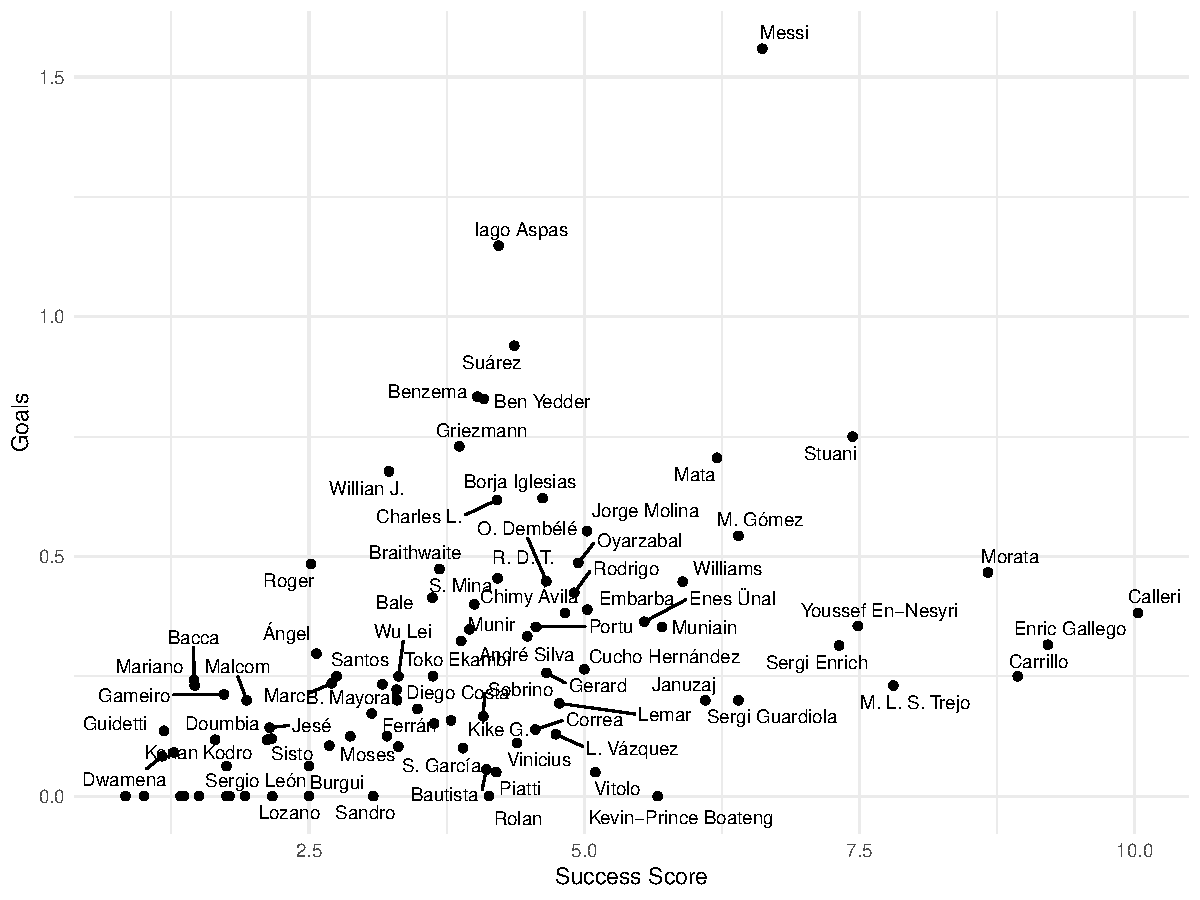
\includegraphics[width=0.8\linewidth]{Assignment-4-ETC5513_files/figure-latex/goals-v-success-1} 

}

\caption{Goals vs Success score}\label{fig:goals-v-success}
\end{figure}

The figure \ref{fig:goals-v-success} is a scatter plot of all the players' goals and success score per game. The players that occur on the top right corner are so far the top players in our analysis. We can see that Messi appears to be one of the top players.

Now that we have analysed all the positives, let's dive into the negatives and see how the players perform. A yellow card is given as a caution when a player is reckless, careless, misconduct, or uses excessive force.

\begin{figure}[H]

{\centering 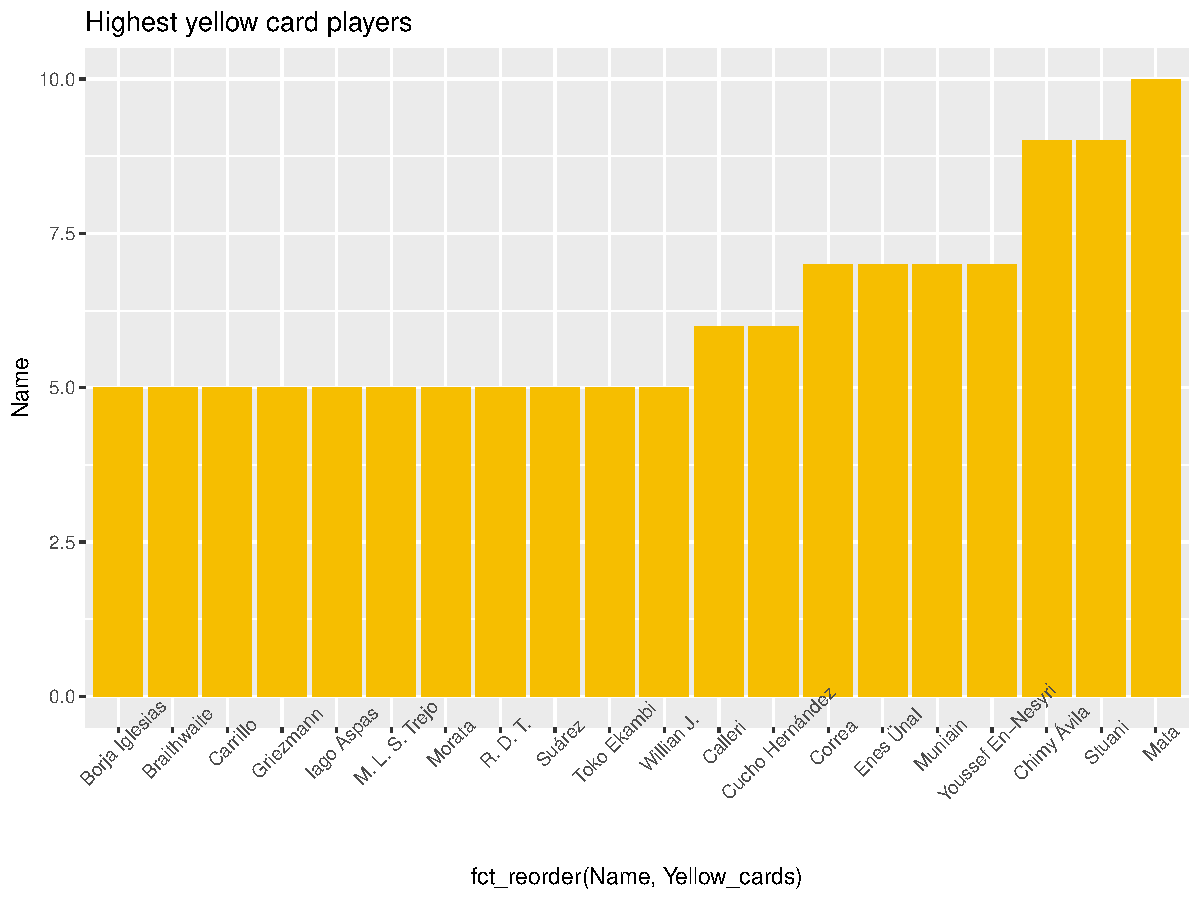
\includegraphics[width=0.8\linewidth]{Assignment-4-ETC5513_files/figure-latex/Yellow-cards-1} 

}

\caption{Top 20 yellow card players}\label{fig:Yellow-cards}
\end{figure}

The figure \ref{fig:Yellow-cards} displays the players with the highest number of yellow cards.

\begin{table}[H]

\caption{\label{tab:Top}Top 5 forward position players}
\centering
\begin{tabular}[t]{l|l}
\hline
Team & Name\\
\hline
FC Barcelona & Messi\\
\hline
RC Celta & M. Gómez\\
\hline
Getafe CF & Jorge Molina\\
\hline
Athletic Club & Williams\\
\hline
SD Huesca & Enric Gallego\\
\hline
\end{tabular}
\end{table}

We will remove the players from the competition of best forward player that have high number of yellow cards.

The table \ref{tab:Top} displays the top 5 forward position players in the LaLiga Tournament according to the 2019-2022 data on the basis of their goals, assists, successful duels and tackles per game and after removing the players with high number of yellow cards. \textbf{\href{images/messi.jpeg}{Messi from FC Barcelona}} is at the top of the list followed by M. Gómez, Jorge Molina, Williams and Enric Gallego.\\

\newpage

\hypertarget{position-midfielder}{%
\section{Position: Midfielder}\label{position-midfielder}}

\hypertarget{aim}{%
\subsubsection{Aim :}\label{aim}}

\begin{itemize}
\item
  Find out the best offensive midfielders in La Liga (2019-2020) and analyze their performance.
\item
  Find out the best defensive midfielders in La Liga (2019-2020) and analyze their performance.
\end{itemize}

Midfielders are the players that are present between the forwards and the defenders. The role of a midfielder is to support both the strikers and the defenders. They act as a link between the offense and defense of a team. The flow of a game is dictated by the midfielders as they are the ones responsible for keeping the ball in possession.

From the table \ref{tab:Attack} we can see the attacking performance of midfielders in La Liga. Sarabia of Sevilla FC stands at the top with 12 goals scored and 13 assists with 33 games played. Every other player has fewer assists than him and only J. Morales from Levante UD was able to match his record of 12 goals.

\begin{table}[H]

\caption{\label{tab:Attack}Best Offensive Midfielders in La Liga (Statistics)}
\centering
\begin{tabular}[t]{l|l|r|r|r|r}
\hline
Team & Name & Shirt.number & Games.played & Goals.scored & Assists\\
\hline
Sevilla FC & Sarabia & 17 & 33 & 12 & 13\\
\hline
Levante UD & J. Morales & 11 & 37 & 12 & 5\\
\hline
Valencia CF & Parejo & 10 & 36 & 9 & 7\\
\hline
Real Betis & Giovani Lo Celso & 21 & 32 & 9 & 4\\
\hline
Athletic Club & Raúl García & 22 & 33 & 9 & 3\\
\hline
Real Betis & Canales & 6 & 32 & 7 & 2\\
\hline
RC Celta & B. Méndez & 23 & 31 & 6 & 7\\
\hline
Real Betis & Joaquín & 17 & 30 & 6 & 0\\
\hline
D. Alavés & Jony & 23 & 36 & 5 & 10\\
\hline
Valencia CF & Gonçalo Guedes & 7 & 25 & 5 & 3\\
\hline
\end{tabular}
\end{table}

The figure \ref{fig:ggAttack} gives a better outlook at the performance of the top midfielders in La Liga. Sarabia and J. Morales standout among their peers as they clearly the leaders in attacking style play, they have scored goals and provided assistance for the benefit of their team. Joaquin from Real Betis is a special case as he is the only midfielder that has provided zero assists but scored 6 goals for his team, earning him a place among the top ten midfielders of La Liga.

\begin{figure}[H]

{\centering 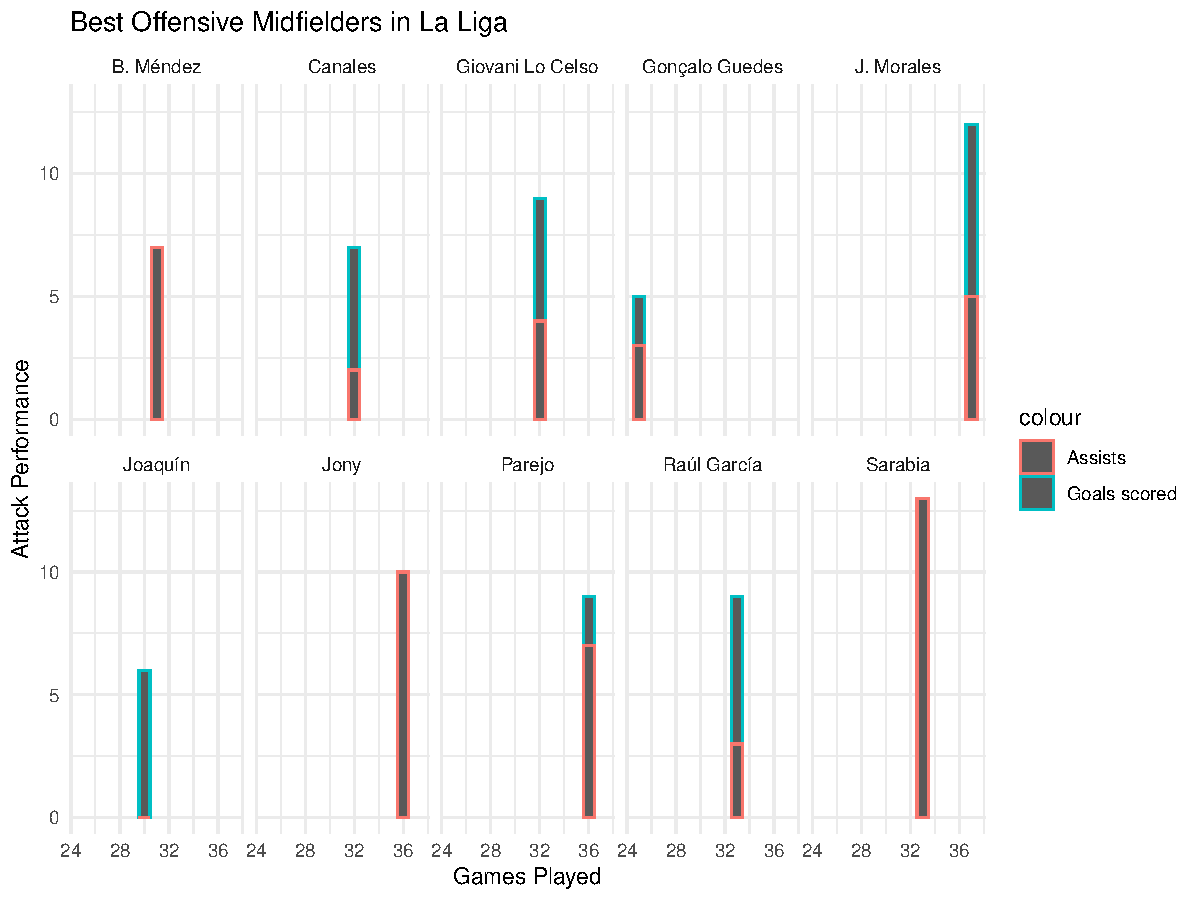
\includegraphics[width=0.8\linewidth]{Assignment-4-ETC5513_files/figure-latex/ggAttack-1} 

}

\caption{Best Offensive Midfielders in La Liga}\label{fig:ggAttack}
\end{figure}

From the table \ref{tab:Defense}, we see the top defensive midfielders in La Liga. Banega from Sevilla FC tops the table, making 290 recoveries and 50 successful tackles in 32 games. Only Rodrigo from Atlético de Madrid has the most successful tackles than Banega standing at 70. None of the other peers have come closer Rodrigo in their skill of tackling an opponent.

\begin{table}[H]

\caption{\label{tab:Defense}Best Defensive Midfielders in La Liga (Statistics)}
\centering
\begin{tabular}[t]{l|l|r|r|r|r}
\hline
Team & Name & Shirt.number & Games.played & Recoveries & Successful.tackles\\
\hline
Sevilla FC & Banega & 10 & 32 & 290 & 50\\
\hline
Atlético de Madrid & Rodrigo & 14 & 34 & 280 & 70\\
\hline
Valencia CF & Parejo & 10 & 36 & 270 & 42\\
\hline
Levante UD & J. Campaña & 24 & 36 & 268 & 45\\
\hline
R. Valladolid CF & Rubén Alcaraz & 14 & 34 & 268 & 54\\
\hline
SD Huesca & Moi Gómez & 6 & 36 & 252 & 28\\
\hline
SD Eibar & Jordán & 24 & 36 & 249 & 40\\
\hline
RCD Espanyol & M. Roca & 21 & 35 & 236 & 45\\
\hline
R. Valladolid CF & Míchel & 21 & 35 & 228 & 38\\
\hline
CD Leganés & Rubén Pérez J. & 21 & 31 & 225 & 42\\
\hline
\end{tabular}
\end{table}

From the figure \ref{fig:ggDefense} we can see that all the defensive midfielders have been almost at the same skill. The top performers Banega and Rodrigo stand out in their individual departments but are almost at the same level as their peers in La Liga. Banega seems to more of a top performer because he is on the top of table even though has played the fewest games 32, except Rubén Pérez J. who has played 31 and is at the bottom of the table.

\begin{figure}[H]

{\centering 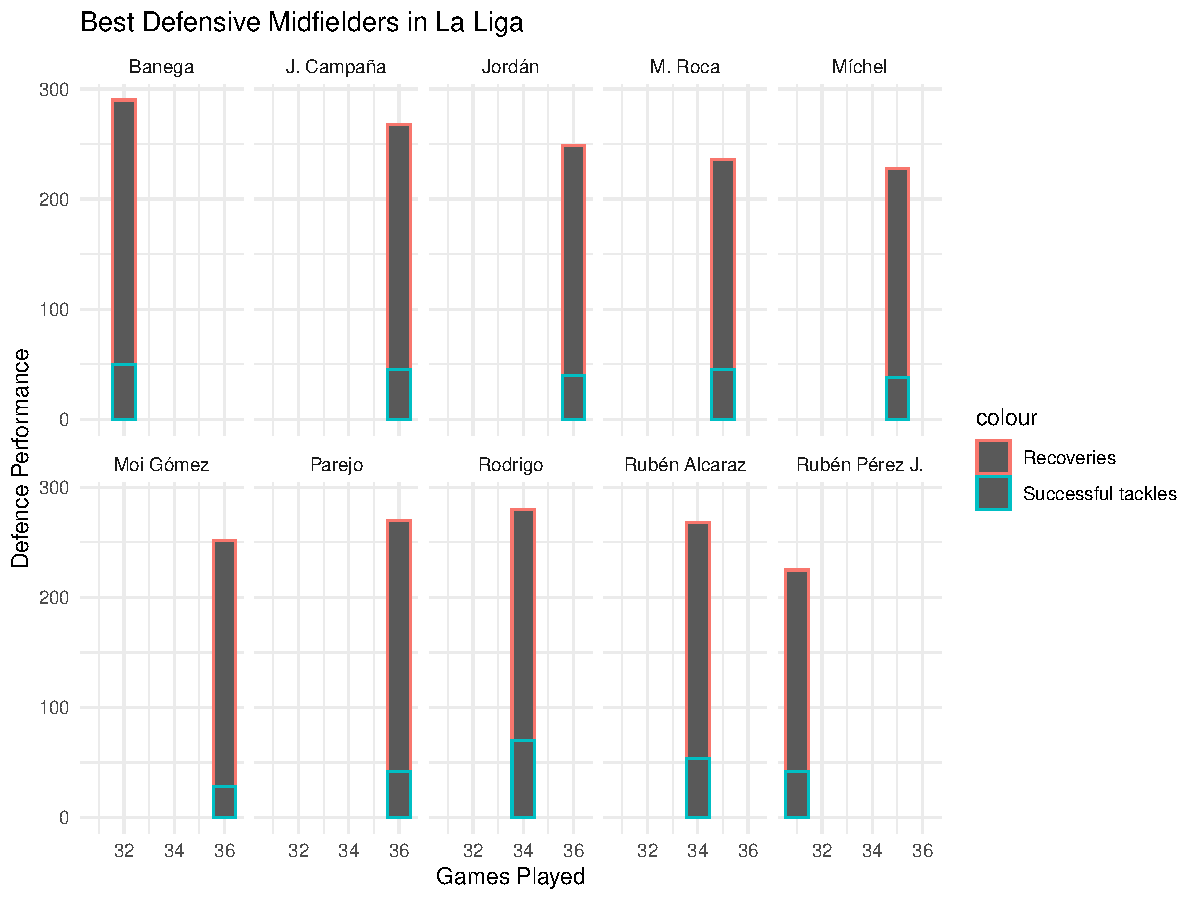
\includegraphics[width=0.8\linewidth]{Assignment-4-ETC5513_files/figure-latex/ggDefense-1} 

}

\caption{Best Defensive Midfielders in La Liga }\label{fig:ggDefense}
\end{figure}

The best overall performance is given by Parejo of Valencia CF as we can from the table \ref{tab:best}. He has made 270 recoveries, 42 successful tackles, scored 9 goals and made 7 assists. He has been at the third position in both offensive midfielders and defensive midfielders. His performance has been exceptional as midfielder and is quite an ideal candidate for any team.

\begin{table}[H]

\caption{\label{tab:best}Best Overall Performace}
\centering
\begin{tabular}[t]{l|l|r|r|r|r|r|r}
\hline
Team & Name & Shirt.number & Games.played & Recoveries & Successful.tackles & Goals.scored & Assists\\
\hline
Valencia CF & Parejo & 10 & 36 & 270 & 42 & 9 & 7\\
\hline
\end{tabular}
\end{table}

\hypertarget{position-goalkeeper}{%
\section{Position : Goalkeeper}\label{position-goalkeeper}}

The Aim of this section is to find out the \textbf{best goalkeeper} in La-Liga (A Spanish football league) in season 2019-2020 according to player stats. We will be performing an analysis to different variables to find out best goalkeeper.

\textbf{Question:}

\textbf{Which football team's goalkeeper has the best performance in La-Liga in the season 2019 - 2020 ?}

\begin{itemize}
\item
  The football term \textbf{``Recoveries''} can be defined as ``Ball recoveries'' stands for recovering the ball in a situation where neither team has possession or where the ball has been played directly to a player by an opponent.
\item
  The football term \textbf{``Clearances''} can be defined as when a goalkeeper kicks the ball away from the goal they are defending
\end{itemize}

Those two terms \textbf{``Recoveries'' and ``Clearances''} are the two main variables we will be focused on for analysis goalkeeper's performance.

\begin{figure}[H]

{\centering 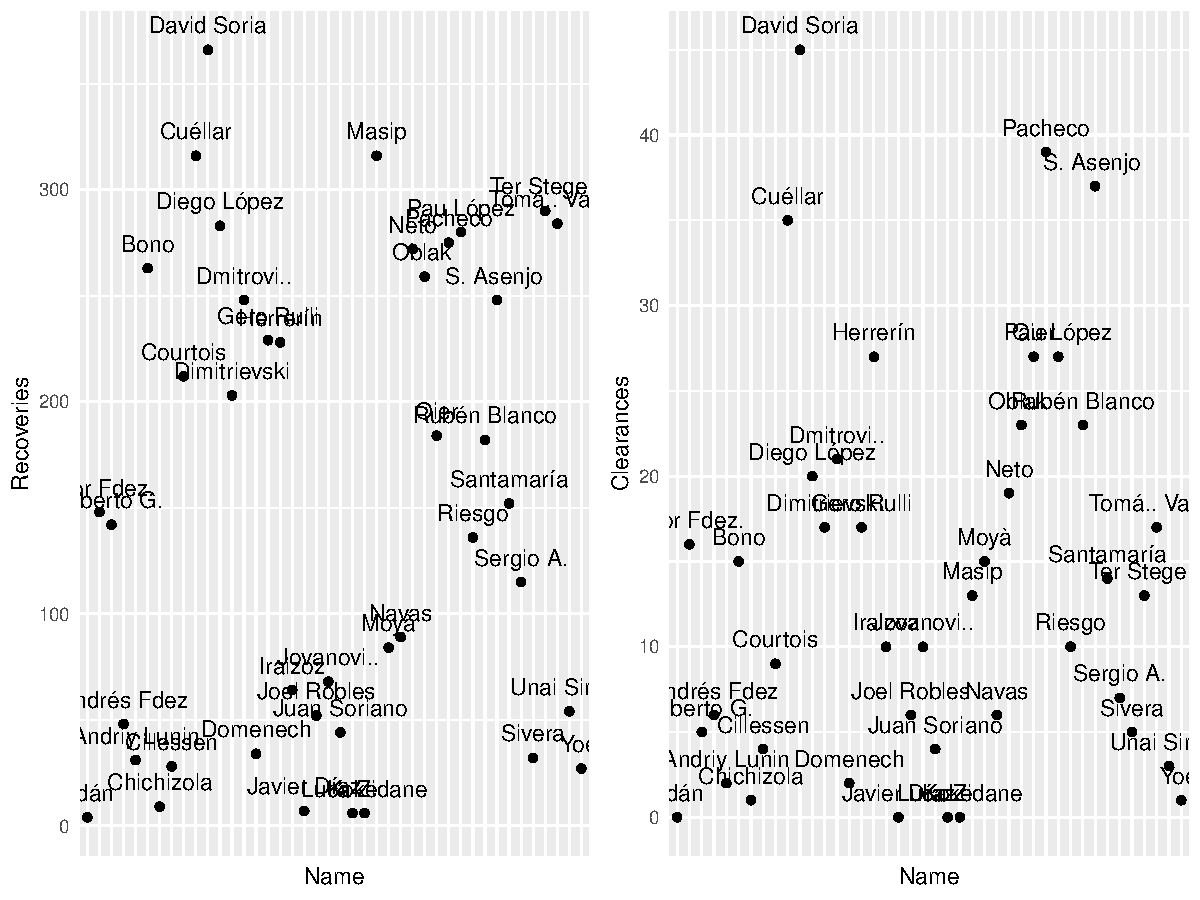
\includegraphics[width=0.8\linewidth]{Assignment-4-ETC5513_files/figure-latex/graph-data-1} 

}

\caption{Recoveries and Clearances}\label{fig:graph-data}
\end{figure}

In Figure \ref{fig:graph-data}, it shows the data of Recoveries and Clearances for each goalkeeper in La-Liga during the season 2019 to 2020.

\begin{figure}[H]

{\centering 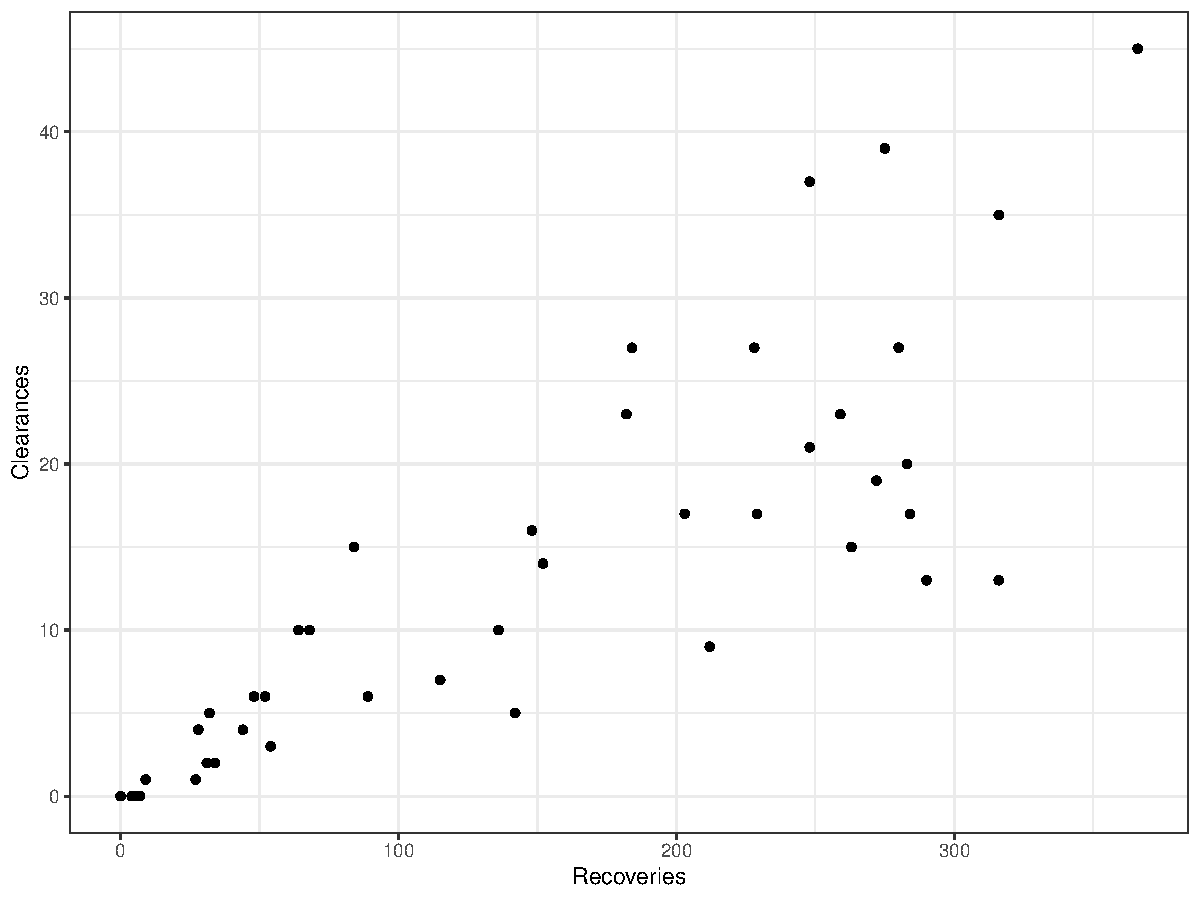
\includegraphics[width=0.8\linewidth]{Assignment-4-ETC5513_files/figure-latex/scatter-plot-1} 

}

\caption{Scatter plot for Recoveries and Clearances}\label{fig:scatter-plot}
\end{figure}

In Figure \ref{fig:scatter-plot}, it displays a scatter plot for goalkeepers' Recoveries and Clearances, it demonstrates there is a positive relationship between variable Clearances and Recoveries.

\begin{longtable}[]{@{}llccr@{}}
\caption{\label{tab:goal-data1}Top 10 Goalkeepers}\tabularnewline
\toprule
Team & Name & Recoveries & Clearances & Rank \\
\midrule
\endfirsthead
\toprule
Team & Name & Recoveries & Clearances & Rank \\
\midrule
\endhead
Getafe CF & David Soria & 366 & 45 & 1 \\
CD Leganés & Cuéllar & 316 & 35 & 2 \\
D. Alavés & Pacheco & 275 & 39 & 3 \\
Real Betis & Pau López & 280 & 27 & 4 \\
Villarreal CF & S. Asenjo & 248 & 37 & 5 \\
RCD Espanyol & Diego López & 283 & 20 & 6 \\
Atlético de Madrid & Oblak & 259 & 23 & 7 \\
Sevilla FC & Tomáš Vaclík & 284 & 17 & 8 \\
Athletic Club & Herrerín & 228 & 27 & 9 \\
Valencia CF & Neto & 272 & 19 & 10 \\
\bottomrule
\end{longtable}

In Table \ref{tab:goal-data1}, it shows the football recoveries and clearances of top 10 goalkeepers in in La-Liga during the season 2019 to 2020.

In this section, the data of goalkeeper has been using to investigate and in a aim to find which goalkeeper is overall performing best in La-Liga during the season 2019 to 2020. The Figure \ref{fig:graph-dat} shows the performance of each single goalkeeper in term of Recoveries and Clearances during the season. In the Figure \ref{fig:scatterplot}, it demonstrates that there is a linear relationship between Recoveries and Clearances, on other words, a goalkeeper tends to have a good performance in term of Recoveries also performing well in term of Clearances. Based on the observation in the scatter plot, Recoveries and Clearances are two standard variables sharing some similarity. Hence, we can rank each variable Recoveries and Clearance and combine the ranks to find the average performance on both Recoveries and Clearances, and then the top 10 goalkeepers are listed out based on the average rank of performance. As displayed on Table \ref{tab:goal-data1}, the goalkeeper David Soria, from football team Getafe CF, is performing best among all goalkeepers in La-Liga during season 2019 - 2020.

\hypertarget{conclusion}{%
\section{Conclusion}\label{conclusion}}

The conclusions from each section were validated and compared with existing research like \textcite{brito2019new} on football players.

\begin{itemize}
\item
  In the first section, there was a tough competition between Gerard Pique and LaGuardia from Barcelona and Alaves respectively \ref{fig:CvsR} . After comparing each of the defenders from the 20 teams on their defensive capabilities \ref{fig:better1} \textbf{Gerard Pique} from Barcelona came out on top.
\item
  To be the best forward in the league you will have to be a great player offensively and they are the players who get the team the three points in every match. After Comparing all the forwards from the league on their offensive capabilities \textbf{Lionel Messi} from Barcelona came out on top as you can also see in \ref{tab:Top} .
\item
  Midfielders are usually a mix of both defenders and forwards as they as they are the Important link between forwards and defenders so they have to Master their skills both offensively and defensively. Keeping in mind these criteria's after our analysis \textbf{D. Parejo} from Valencia CF has all the required skills to be the best midfielder in the season 19-20. \ref{tab:best}
\item
  Lastly, a goalkeeper is the backbone of the team as he is our last defender and the first attacker, \textbf{David Soria} from Getafe had the most impact as a goalkeeper on the team. \ref{tab:goal-data1}
\end{itemize}

\printbibliography

\end{document}
